% !TEX root = ../proposal.tex
%
\chapter{Objectives}
\label{sec:objectives}

For reasons described in \cref{sec:motivation}, the goal of the thesis is to design, implement and validate an experimentation system for implicit user feedback with a more holistic view on the problem than in existing publications.
Using this system, it shall be possible to visualise and analyse implicit user feedback that was previously supplied to its storage layer.
In order to accomplish this task, a system as pictured in \cref{fig:system:vision} has to be implemented.
The concrete goals are as follows:

\begin{enumerate}
\item Classify existing solutions / approaches for establishing passive user feedback.
\item Design and implement a system that allows the collection of passive user feedback with considerably low effort.
This part of the system is comprised of the storage layer, an aggregation service and a hypothetical client application which logs events to storage whenever the user performs certain actions (cf. 4.).
%It also features two users: The end user of the client application, and the analyst who wants to evaluate the user feedback.
These events can be purely UI related, such as click or hover events, but some will also be related to the business logic, like executing transactions or creating content.
In order to forward the user feedback data to the analysis application (cf. 3.), the aggregation service has to fetch the appropriate data from the store.
While making use of a caching mechanism during this step would certainly make sense, such a feature will presumably not be part of the final solution due to the additional complexity; if this is the case, the system shall be easily extensible for introducing such a feature.
This objective involves researching and assessing fitting infrastructure and tooling solutions.
\item Design this system such that it also allows analysis of collected user feedback, and implement this as well.
When someone wants to evaluate the collected user feedback via the analysis application, the application shall display data, which it fetches from the aggregation service.
The best approach for displaying the data has yet to be evaluated, but will involve some graphical representation in form of charts and / or graphs.
This objective also implicates research and choosing of appropriate solutions that shall be used for this part of the system.
\item Evaluate how this system performs, which involves collecting user feedback and analysing it.
Implementation of the client application itself will not be done for the purpose of this thesis.
Instead, some existing application shall be extended in order to log the appropriate events, or an existing data set such as the one presented by \citet{Deka:2017:Rico} shall be used.
In the latter case, some application or script has to be written which imports the needed UI interaction data to the event store.
\item As an additional requirement, the experimentation system shall be platform independent, i.e. run on the most widely used operating systems Linux, MacOS and Windows.
\end{enumerate}

\begin{figure}[htb]
        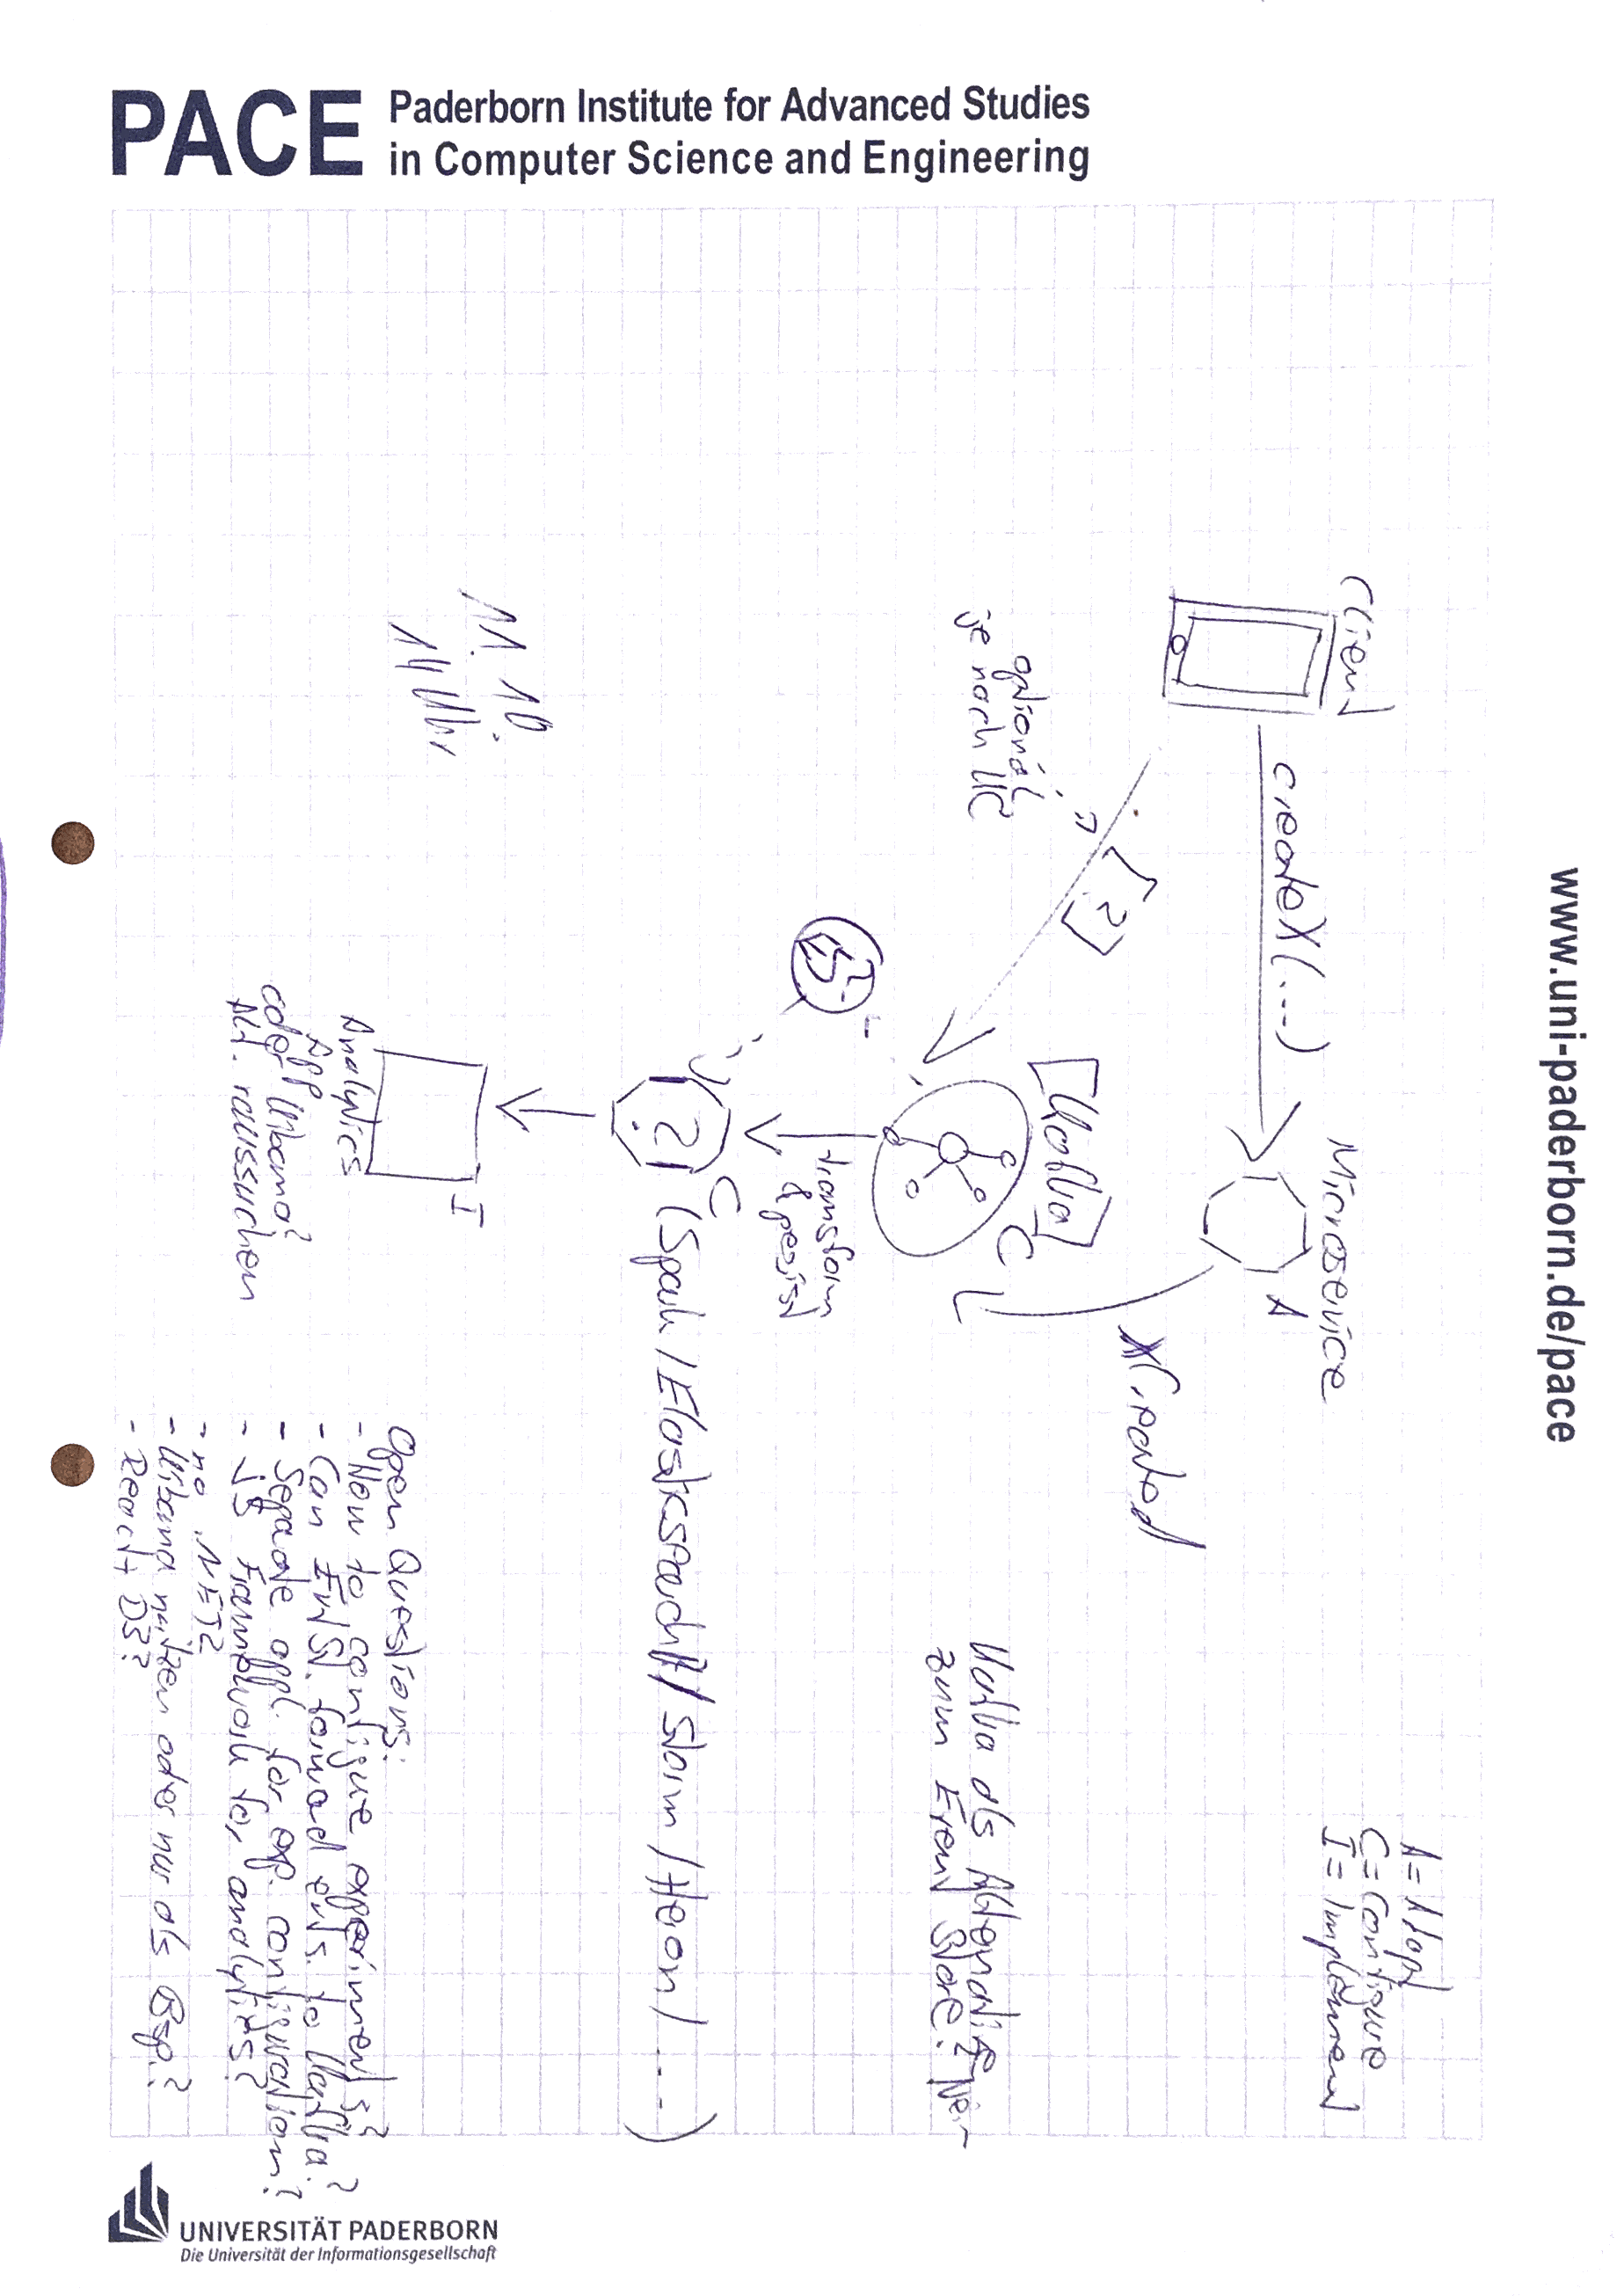
\includegraphics[width=\textwidth]{gfx/architecture-1}
        \caption{The envisioned architecture of the experimentation system.}
        \label{fig:system:vision}
\end{figure}
